\documentclass[11pt]{article}
\usepackage{geometry}                % See geometry.pdf to learn the layout options. There are lots.
\geometry{letterpaper}                   % ... or a4paper or a5paper or ... 
%\geometry{landscape}                % Activate for for rotated page geometry
%\usepackage[parfill]{parskip}    % Activate to begin paragraphs with an empty line rather than an indent
\usepackage{graphicx}
\usepackage{amssymb}
\usepackage{amsmath}
\usepackage{epstopdf}
\usepackage{hyperref}
\DeclareGraphicsRule{.tif}{png}{.png}{`convert #1 `dirname #1`/`basename #1 .tif`.png}



\graphicspath{
{/Users/Andy/Cruises_Research/Analysis/Andy_Pickering/tiwe_patch_gamma/figures/}
}

\title{Patch/Gamma Analysis for TIWE chameleon patches}
\author{Andy Pickering}
%\date{}                                           % Activate to display a given date or no date



\begin{document}
\maketitle

\tableofcontents
\newpage

%~~~~~~~~~~~~~~~~~~~~~
\section{Overview}

The goal of this analysis is to estimate the mixing coefficent ($\gamma_{\chi\epsilon}=\frac{N^2 \chi}{2\epsilon T_{z}^{2}} $) for patches in TIWE chameleon profiles, and see if we obtain values close to the normally-assumed $\gamma=0.2$. Results are also compared to previous estimates used in Smyth et al 2001.

%~~~~~~~~~~~~~~~~~~~~~
\section{Data}

Data are made by the `Chameleon' microstructure profiler near the equator during the `TIWE' experiment. Data was shared by JN and my local copy is at: \newline \verb+/Users/Andy/Dropbox/AP_Share_With_JN/date_from_jim/Tiwe91+

\medskip

I'm using the raw Chameleon data files in: \newline
\verb+/Users/Andy/Dropbox/AP_Share_With_JN/date_from_jim/Tiwe91/cham/tw/+

\medskip

All my analysis is in the main folder: \newline  \verb+/Users/Andy/Cruises_Research/ChiPod/TIWE+


%~~~~~~~~~~~~~~~~~~~~~
\section{Methods}

\begin{itemize}

\item \verb+Run_tiwe_AP.m+ Runs the standard Chameleon processing, producing 1m avg quantities. I modifed this from \verb+run_tw91.m+.

\item \verb+Combine_tiwe_avg_profiles.m+ Combines the avg profiles made in \verb+Run_tiwe_AP.m+ into a single structure with common depths.

\item \verb+Process_tiwe_rawprofiles_AP.m+  Processes raw Chameleon files and saves `cal2' files which have the raw/ high-res profiles of temp and salinity. These are used to identify patches. $\chi$ and $\epsilon$ are not computed for these.

\item \verb+FindPatches_tiwe_Raw.m+ Identifies patches in each profiles made by \verb+Process_tiwe_rawprofiles_AP.m+, using potential temperature.

\item \verb+Compute_N2_dTdz_patches_tiwe_eachcast.m+ Computes $N^2$ and $T_z$ for patches, using several different methods. Saves results for each profile in a structure `patches'.

\item \verb+add_binned_to_patches.m+ Adds the binned (ie the standard 1m avg values) $\chi$ and $\epsilon$ to the profiles of patches at patch locations. Binned profiles are interpolated to patch depths.

\item \verb+Run_tiwe_AP_forPatches.m+ Runs the Chameleon processing (including $\chi$ and $\epsilon$) for just the patches identified in \verb+FindPatches_tiwe_Raw.m+ . This calls \verb+average_data_PATCH_AP.m+ instead of \verb+average_data_gen1.m+.

\item \verb+add_patch_chi_eps_to_patches_tiwe_each_profile.m+ adds the values of $\chi$ and $\epsilon$ from \verb+Run_tiwe_AP_forPatches.m+ to the patch profiles.

\item \verb+combine_patch_profiles.m+ combines all the individual patch profiles into a single structure.


\end{itemize}

\medskip

%~~~~~~~
\subsection{Overturns}

Overturns (patches) are detected for each profile, using potential temperature (because salinity was noisy/spiky, see later section). The function \verb+compute_overturns_discrete_AP.m+ was used to identify patches. \newline
The following criteria were also applied:
\begin{itemize}
\item Values of $\epsilon <0.4\times 10^{-9}$ were NaN'ed out, following the methods of Smyth et al 2001. Note the paper says $4\times 10^{-9}$ but I think that was a type based on looking at the data Bill sent me.
\item Smyth et al 2001 used a minimum patch size of 15cm, and any patches separated by less than 15cm were joined together.  We use a 40cm minimum in order to be able to calculate calculate accurate $\chi$ and $\epsilon$ from spectra.
\item Only patches in the depth range 60-200m were used (as in Smyth et al 2001). This excludes mainnly buoyancy-driven turbulence associated with the diurnal cycle.
\item For each patch, a linear fit is performed of salinity vs temperature and $R^2$ is computed to quantify how clear the T-S relationship is. We examine the results both with and without a minimum $R^2$ criterion
\end{itemize}


%~~~~~~~
\subsection{dTdz}

Temperature gradient is computed for each patch using the following methods:
\begin{enumerate}
\item $dtdz_{line}$ : Fit a straight line to sorted potential temperature using \verb+polyfit+
\item $dtdz_{bulk}$ : Use the 'bulk gradient' from Smyth et al 2001, which is the rms fluctuation from the background (sorted) temperature, divided by the thorpe scale (the rms re-ordering distances).
\end{enumerate}


%~~~~~~~
\subsection{N2}

$N^2$ is computed for each patch using the following methods:
\begin{enumerate}
\item $N^2_{line}$ : Fit a straight line to sorted potential density using polyfit to get $d\rho/dz$, then compute N2.
\item $N^2_line_fit$ : Salinity/density are computed from the T-S fit.  Then $N^2$ is computed from the sorted density by fitting a line.
\item $N^2_{bulk}$ : Use 'bulk gradient' . This is calculated from the bulk $T_z$, using a linear fit between density and temperature in each patch.
\item $N^2_4$ : Compute $N^2$ from the sorted profile (sorted by potential density) using \verb+sw_bfreq+, then take average over the patch. I believe this method is used by some commonly-used overturn codes.
\end{enumerate}


%~~~~~~~
\subsection{Mixing coefficient (Efficiency)}

Mixing coefficient $\gamma_{\chi\epsilon}$ (often referred to as efficiency) is computed from the following equation using differerent $N^2$ and $dT/dz$ values.
\begin{equation}
\gamma_{\chi\epsilon}=\frac{N^2 \chi}{2\epsilon T_{z}^{2}} 
\end{equation}
$\chi$ and $\epsilon$ are computed over each patch from the Chameleon data. $\gamma_{\chi\epsilon}$ is computed for the following 4 combinations:
\begin{enumerate}
\item  $\gamma_{bin}$ : Binned (1m) $\gamma$ interpolated to patch depths.
\item  $\gamma_{line}$ : $N^{2}_{line}$, $dtdz_{line}$
\item  $\gamma_{bulk}$ : $N^{2}_{bulk}$, $dtdz_{bulk}$
\item  $\gamma_{range}$ : $N^{2}_{4}$, $dtdz_{line}$
\end{enumerate}



%~~~~~~~~~~~~~~~~~~~~~
\section{Results}


\begin{itemize}
\item Figure \ref{1mavgsum} shows a summary of the 1m-binned data. Ydays 324-327 correspond to cast numbers 2836 : 3711. For some reason many $\chi$ values below 150db are bad/missing? Not sure why.
\item The median $\gamma_{\chi\epsilon}$ computed using the 1m avg data is $0.063$ (Figure \ref{avggam})}.
\item Median patch values of $\gamma$ are given in table \ref{tab} and histograms in Figure \ref{patchgam}.
\end{itemize}



\begin{table}[htdp]
\caption{Statistics for patches using various parameters. $\gamma$ values are medians for each distribution. Only patches between 60-200m and on yday 324-327 are considered for all.}
\begin{center}
\begin{tabular}{|c|c|c|c|c|c|c|c|}
\hline
minOT & usetemp & minR2 & $\gamma bin$ & $\gamma line$ & $\gamma fit$ & $\gamma bulk$ & Npatches \\
\hline
0.4 & 1 & 0 & 0.13 & 0.57 & 0.11 & 0.53 & 16329 \\
\hline
0.4 & 1 & 0.5 & 0.14 & 0.22 & 0.12 & 0.21 & 3761 \\
\hline
0.75 & 1 & 0 & 0.15 & 0.62 & 0.14 & 0.59 & 9175 \\
\hline
0.75 & 1 & 0.5 & 0.15 & 0.25 & 0.16 & 0.26 & 2358 \\
\hline
1 & 1 & 0 & 0.16 & 0.71 & 0.15 & 0.68 & 6893 \\
\hline
1 & 1 & 0.5 & 0.16 & 0.29 & 0.17 & 0.29 & 1779 \\
\hline
\hline
\end{tabular}
\end{center}
\label{tab}
\end{table}%


\begin{figure}[htbp]
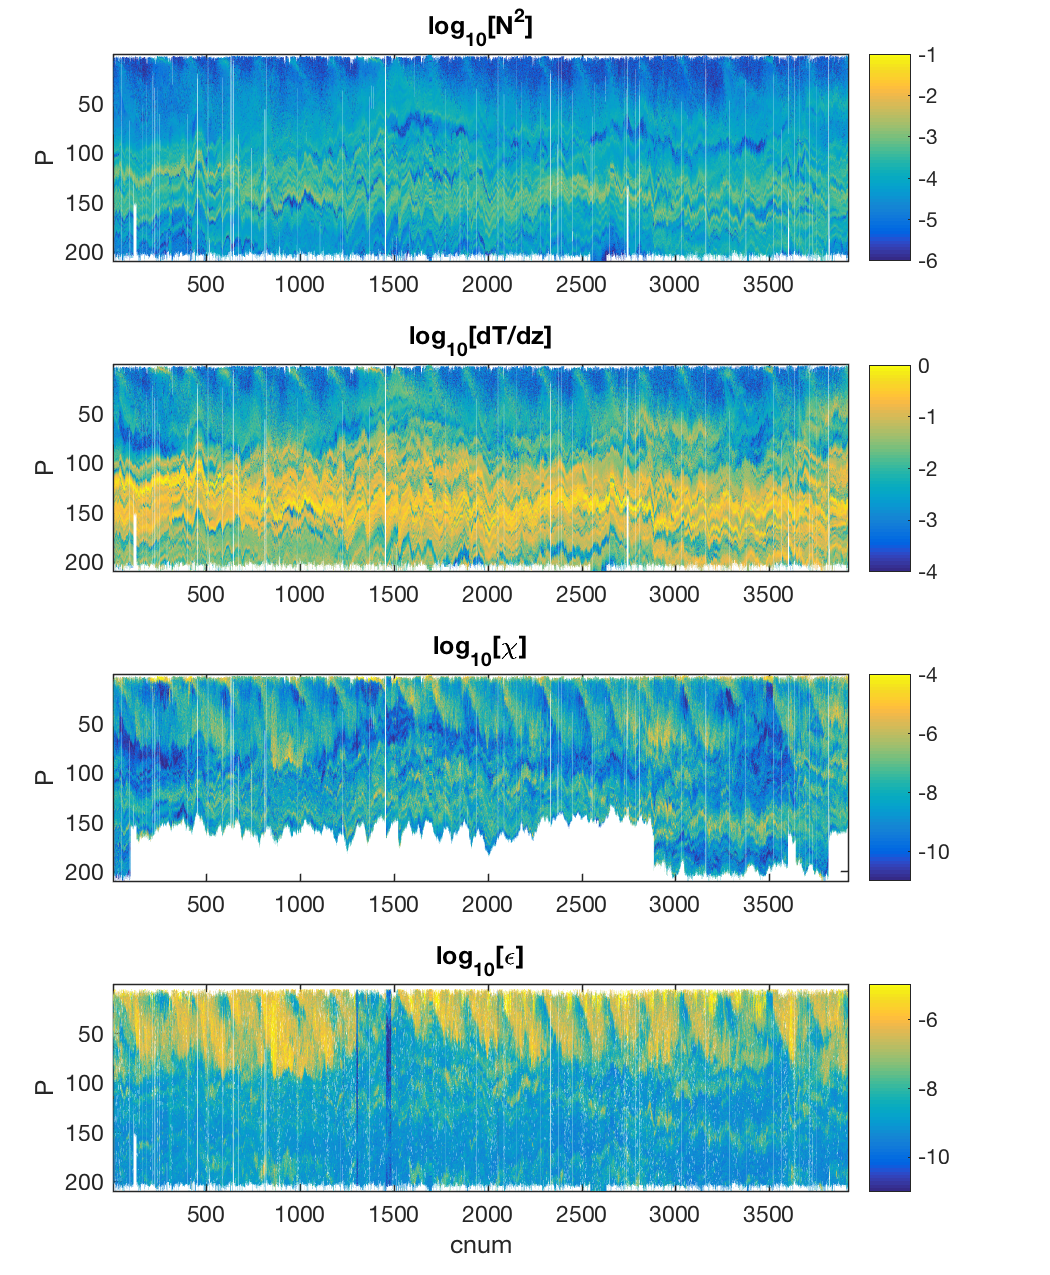
\includegraphics[scale=0.8]{tiwe_avgCombine_N2_dtdz_chi_eps.png}
\caption{Pcolor of the combined 1m avg chameleon data for TIWE. * Note for some reason many $\chi$ values below 150db are bad/missing.}
\label{1mavgsum}
\end{figure}



\begin{figure}[htbp]
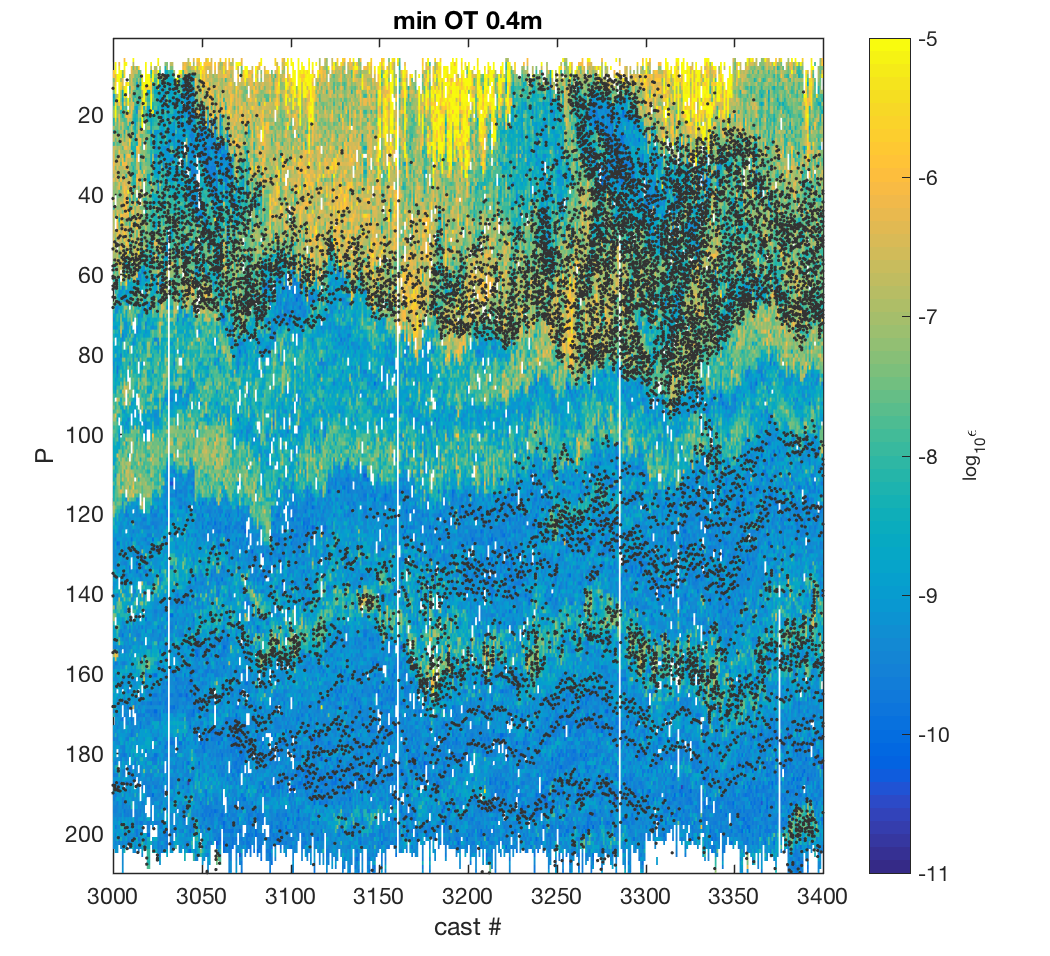
\includegraphics[scale=0.8]{tiwe_minOT_40_usetemp_1_patch_locs.png}
\caption{Pcolor of the combined 1m avg chameleon epsilon for TIWE, and patch locations for a period between yday 324-327. Patches above 60m have not been discarded yet.}
\label{patchlocs}
\end{figure}



% binned gammas
\begin{figure}[htbp]
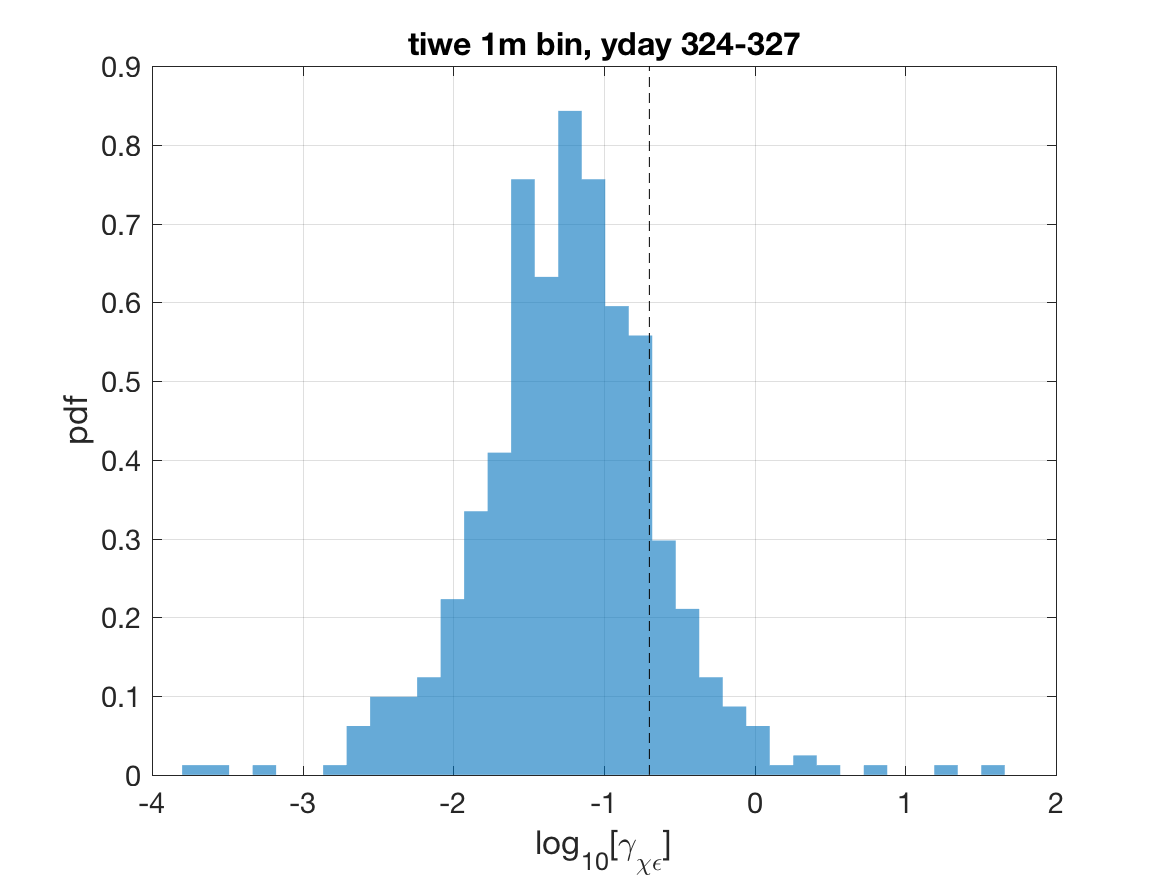
\includegraphics[scale=0.8]{tiwe_avgCombine_gamma_yday_324_327.png}
\caption{Histogram of $\gamma_{\chi\epsilon}$ for 1m avg chameleon profiles on yday 324-327, between 60-200m(no patch analysis applied). Vertical dashed line shows $\gamma_{\chi\epsilon}=0.2$.}
\label{avggam}
\end{figure}


% patch gammas
\begin{figure}[htbp]
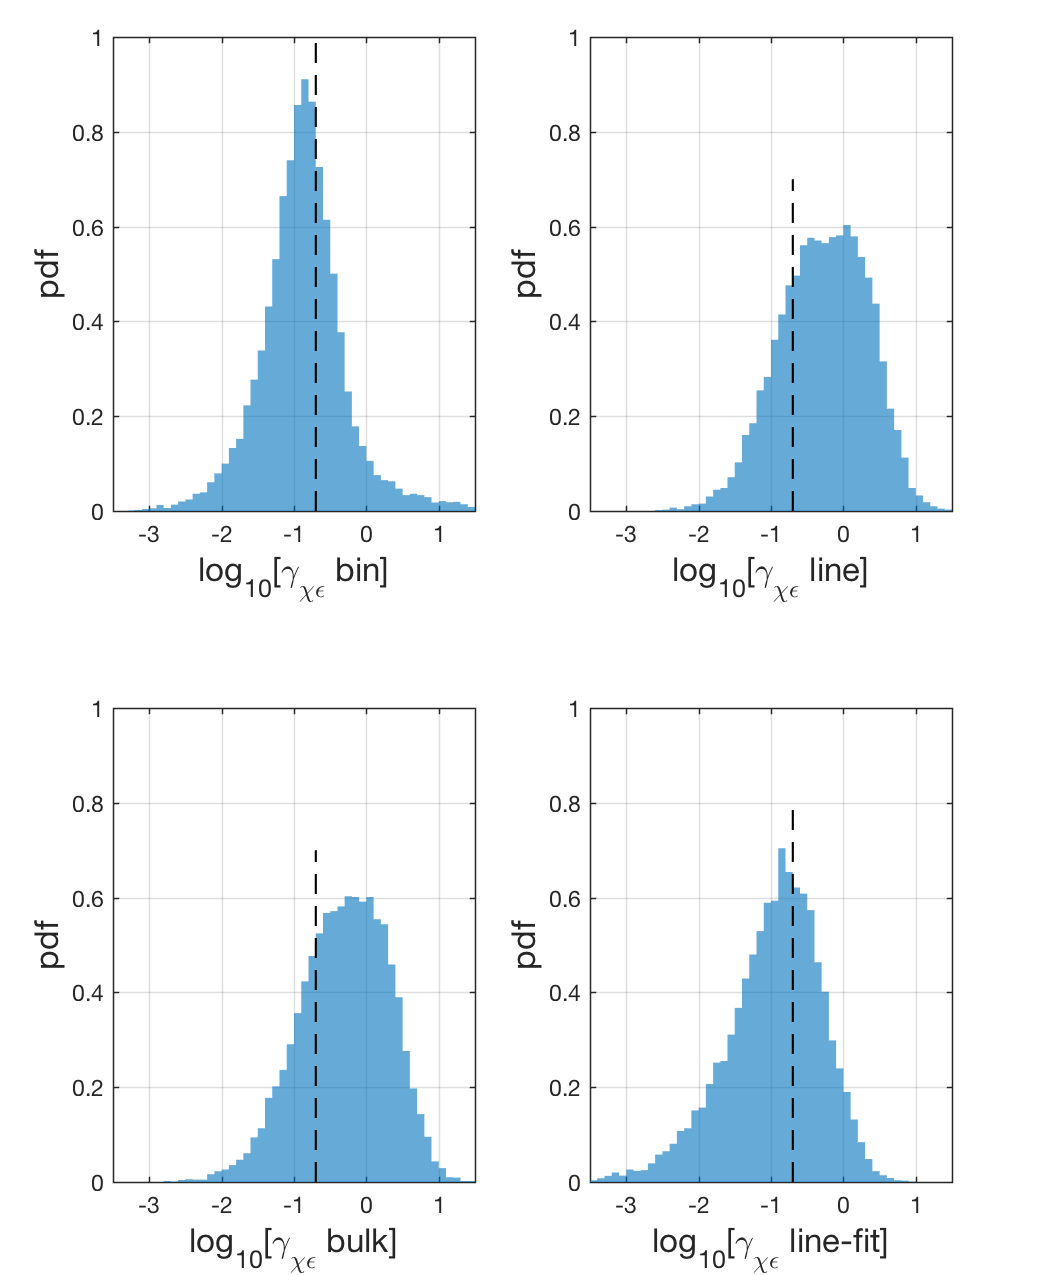
\includegraphics[scale=0.8]{tiwe_minOT_40_usetemp_1_gammas_hist2X2_yday_324_327.png}
\caption{Histogram of $\gamma_{\chi\epsilon}$ for patches using temperature and min OT size of 40cm, using different estimates of $N^2$ and $T_z$. Vertical dashed line shows $\gamma_{\chi\epsilon}=0.2$. Data for profiles on yday 324-327 (corresponding to data used in Smyth et al).}
\label{patchgam}
\end{figure}



\clearpage
%~~~~~~~~~~
\subsection{Temp vs Density}

Comparing overturns compute from temperature vs those computed vs density. Ideally we would use density, but salinity in this dataset looks very noisy/spiky, which could introduce false overturns. Using temperature would avoid this, but only works if there is a tight T-S relationship. This does not appear to be the cast here (Figure \ref{TSplot}). Manual inspection fo some profiles also showed overturns that were identified in temperature, but were stable in density due to the influence of salinity. So what to do? Use density, but smooth or lowpass filter salinity? Or use a larger minimum overturn size ?

% figure showing T-S relationship
\begin{figure}[htbp]
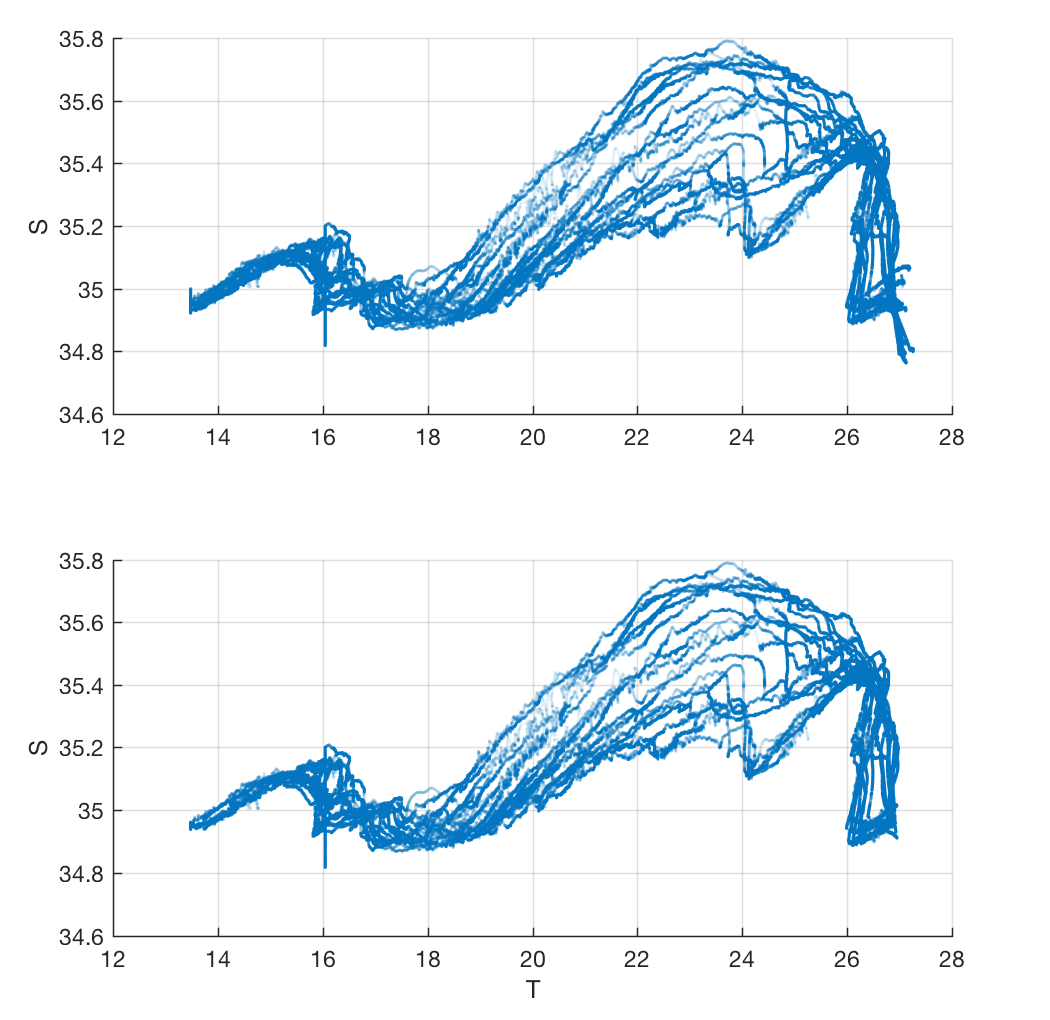
\includegraphics[scale=0.8]{tiwe_T_S_scatter.png}
\caption{ Raw T vs S for a subset of TIWE Chameleon profiles between yday 324-327 (corresponding to data used in Smyth et al).}
\label{TSplot}
\end{figure}




%
%\clearpage
%%~~~~~~~~~~
%\subsection{Different min OT sizes}
%
%The analysis was run for different minimum overturn sizes; here I compare the results.
%
%\begin{itemize}
%\item Doesn't seem to make a difference for the binned estimates of $\gamma$ (1m binned values interpolated to patch locations).
%\item It does make a significant difference when $\gamma$ is computed over each patch. Patches computed from temperature tend to have larger estimated $\gamma$.
%\end{itemize}
%
%
%
%\begin{figure}[htbp]
%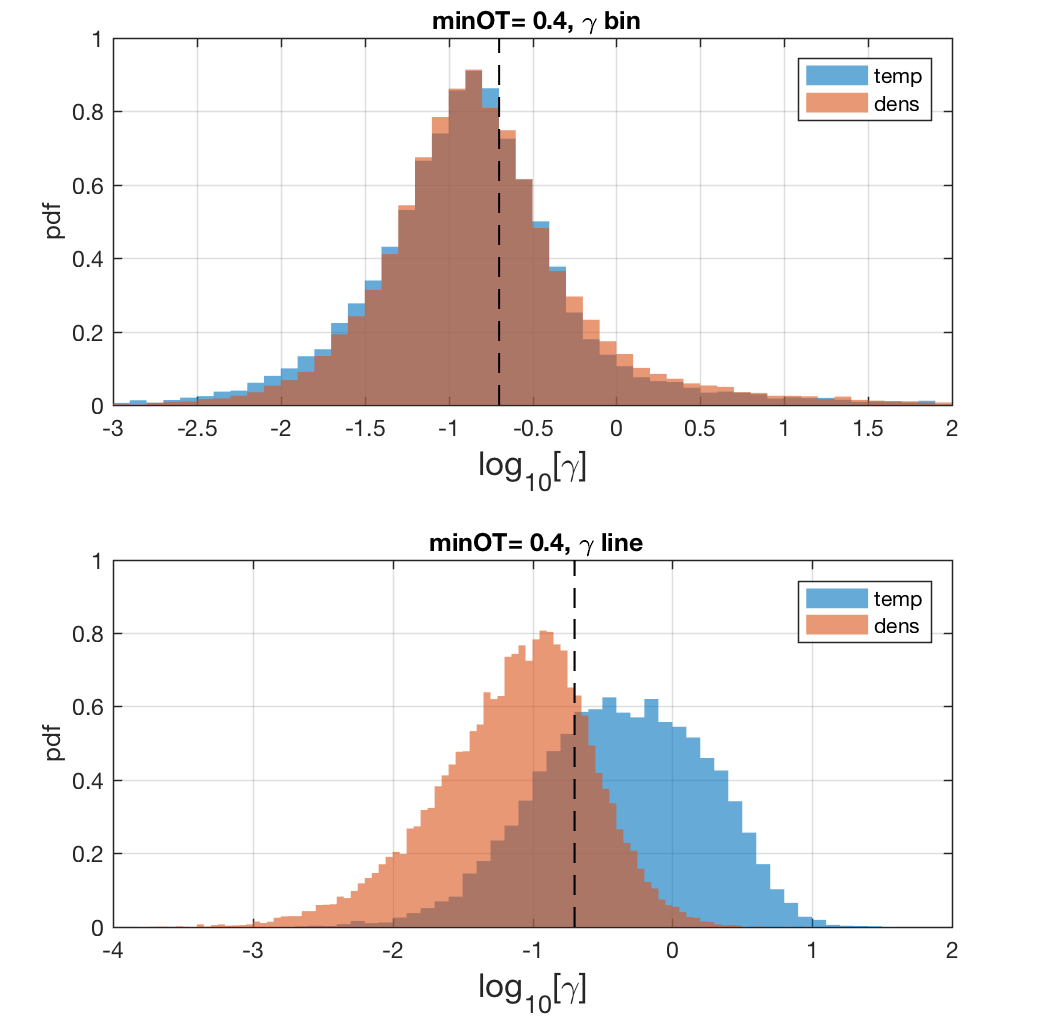
\includegraphics[scale=0.8]{tiwe_minOT_40_gam_TvsD.png}
%\caption{ Comparison of $\gamma$ for patches with minimum size 40cm, computed from temperature vs density.}
%\label{}
%\end{figure}
%
%\begin{figure}[htbp]
%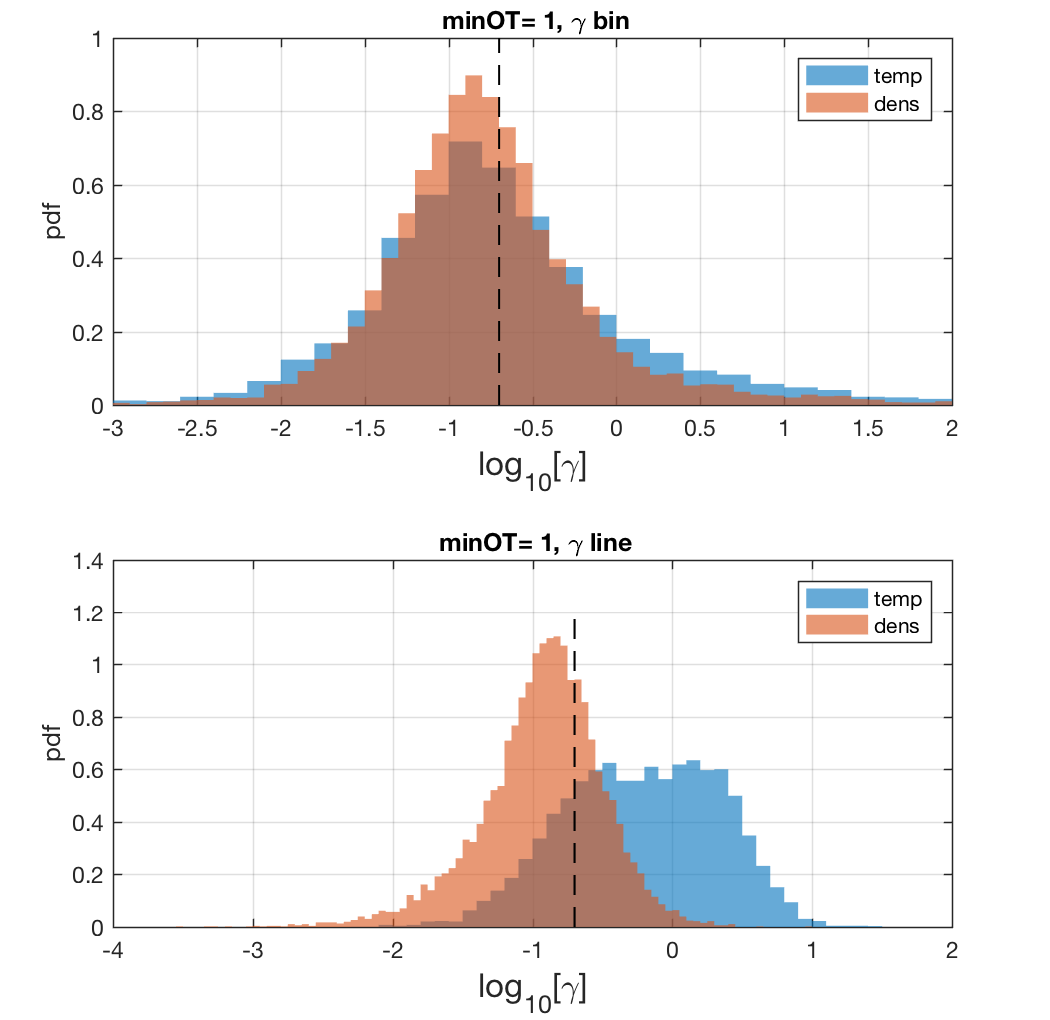
\includegraphics[scale=0.8]{tiwe_minOT_100_gam_TvsD.png}
%\caption{ Comparison of $\gamma$ for patches with minimum size 1m, computed from temperature vs density.}
%\label{}
%\end{figure}
%








\clearpage
%~~~~~~~~~~
\subsection{$\gamma$ vs depth}


\begin{figure}[htbp]
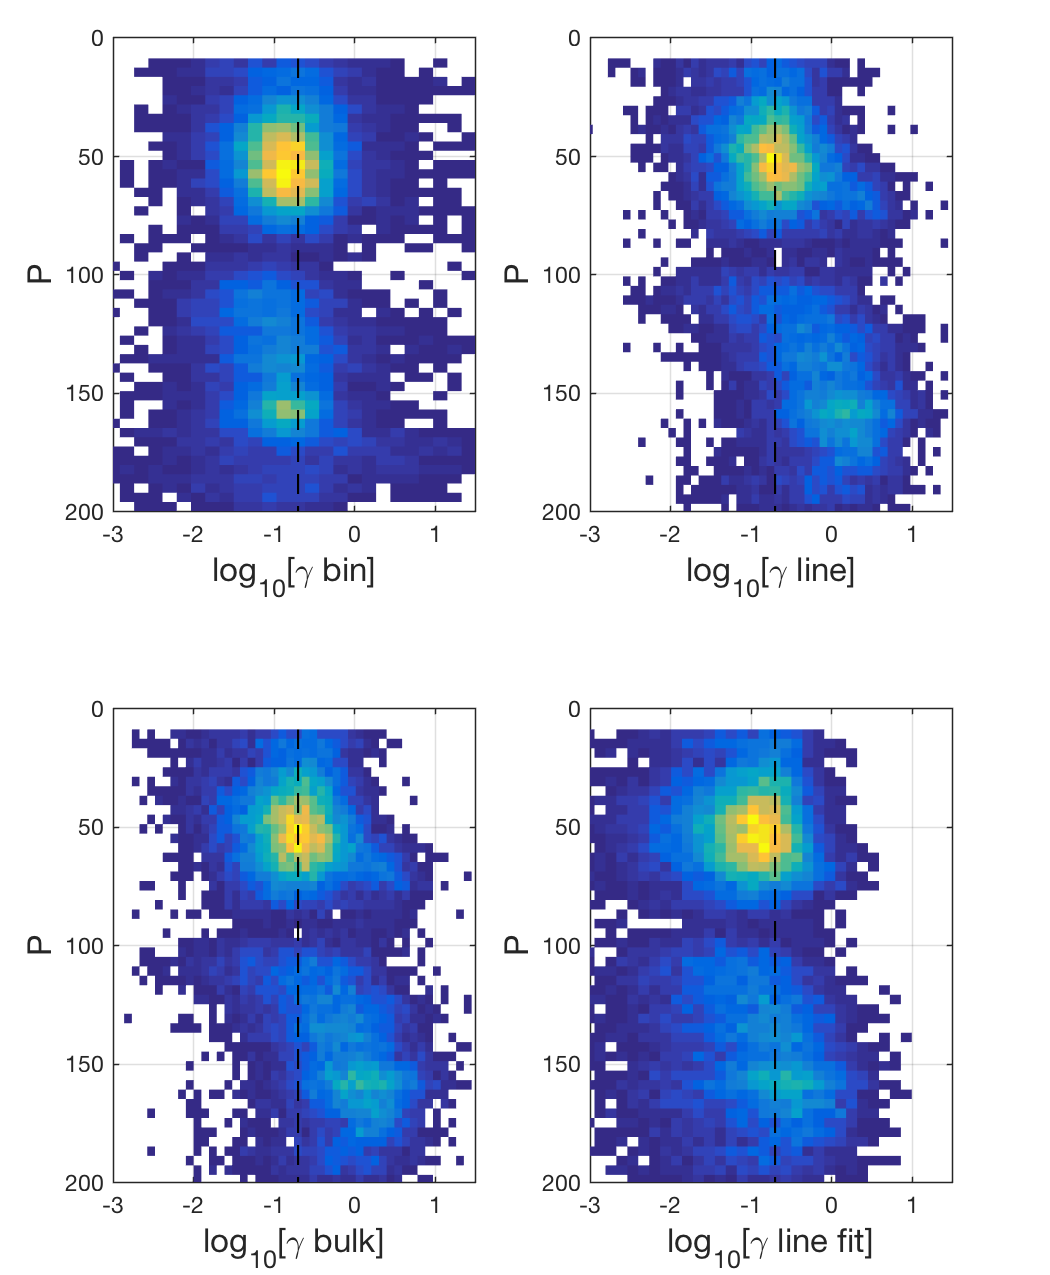
\includegraphics[scale=0.8]{tiwe_minOT_40_usetemp_1_gammas_vs_depth2X2_324_327.png}
\caption{Plot of $\gamma_{\chi\epsilon}$ vs depth for patches identified from temperature with min OT size 40cm. Vertical dashed line shows $\gamma_{\chi\epsilon}=0.2$. Data for profiles on yday 324-327 (corresponding to data used in Smyth et al).}
\label{patch_gam_vs_depth}
\end{figure}


\clearpage
%~~~~~~~~~~
\subsection{$\gamma$ vs $\epsilon$}


\begin{figure}[htbp]
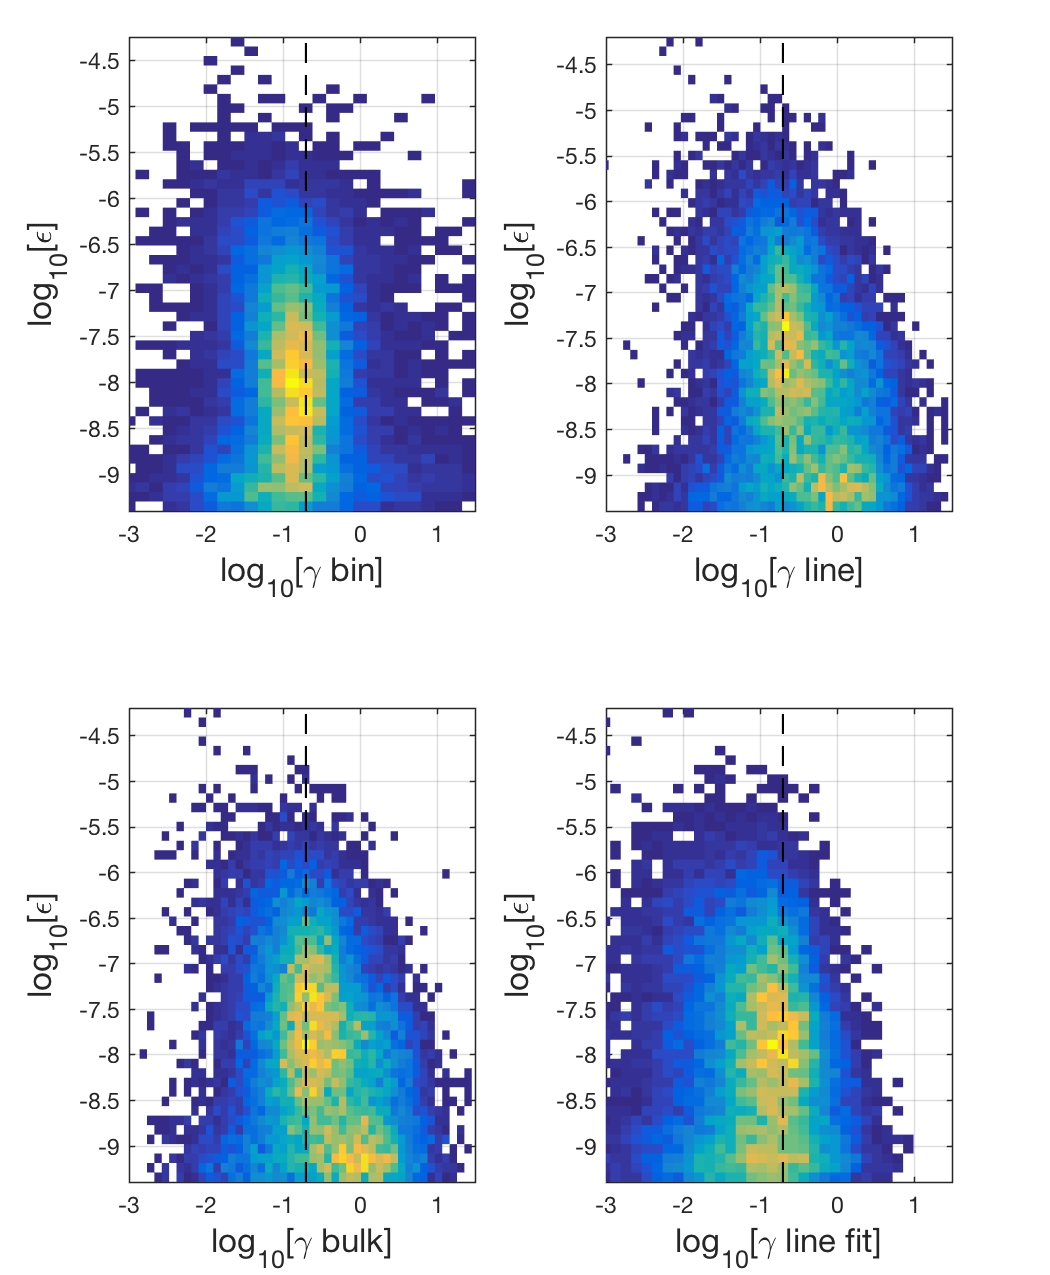
\includegraphics[scale=0.8]{tiwe_minOT_40_usetemp_1_gammas_vs_eps2X2_324_327.png}
\caption{Plot of $\gamma_{\chi\epsilon}$ vs $\epsilon$ for patches computed from temperature with min OT size 40cm. Vertical dashed line shows $\gamma_{\chi\epsilon}=0.2$. Data for profiles on yday 324-327 .}
\label{patch_gam_vs_eps}
\end{figure}





\clearpage
%~~~~~~~~~~~~~~~~~~~~~
\section{Comparison to previous analysis}

Bill send me results of a previous patch analysis for tiwe: \verb+events_TIWE.mat+ . Here i'll compare my results to those. His dataset contains 1155 patches, with a mean $\gamma$ of 0.45 . See \verb+compare_patches_tiwe_AP_Bill.m+ . It looks like my values of $T_z$, and $\chi$ tend to be significantly smaller than Bill's (Figure \ref{comp_bill_ap_1}).% Gamma computed from my patch values (using all profiles) is smaller than 0.2 (median 0.08), while gamma from Bill's values is larger than 0.2 (median 0.4),(Figure \ref{comp_bill_ap_gam}).

\begin{figure}[htbp]
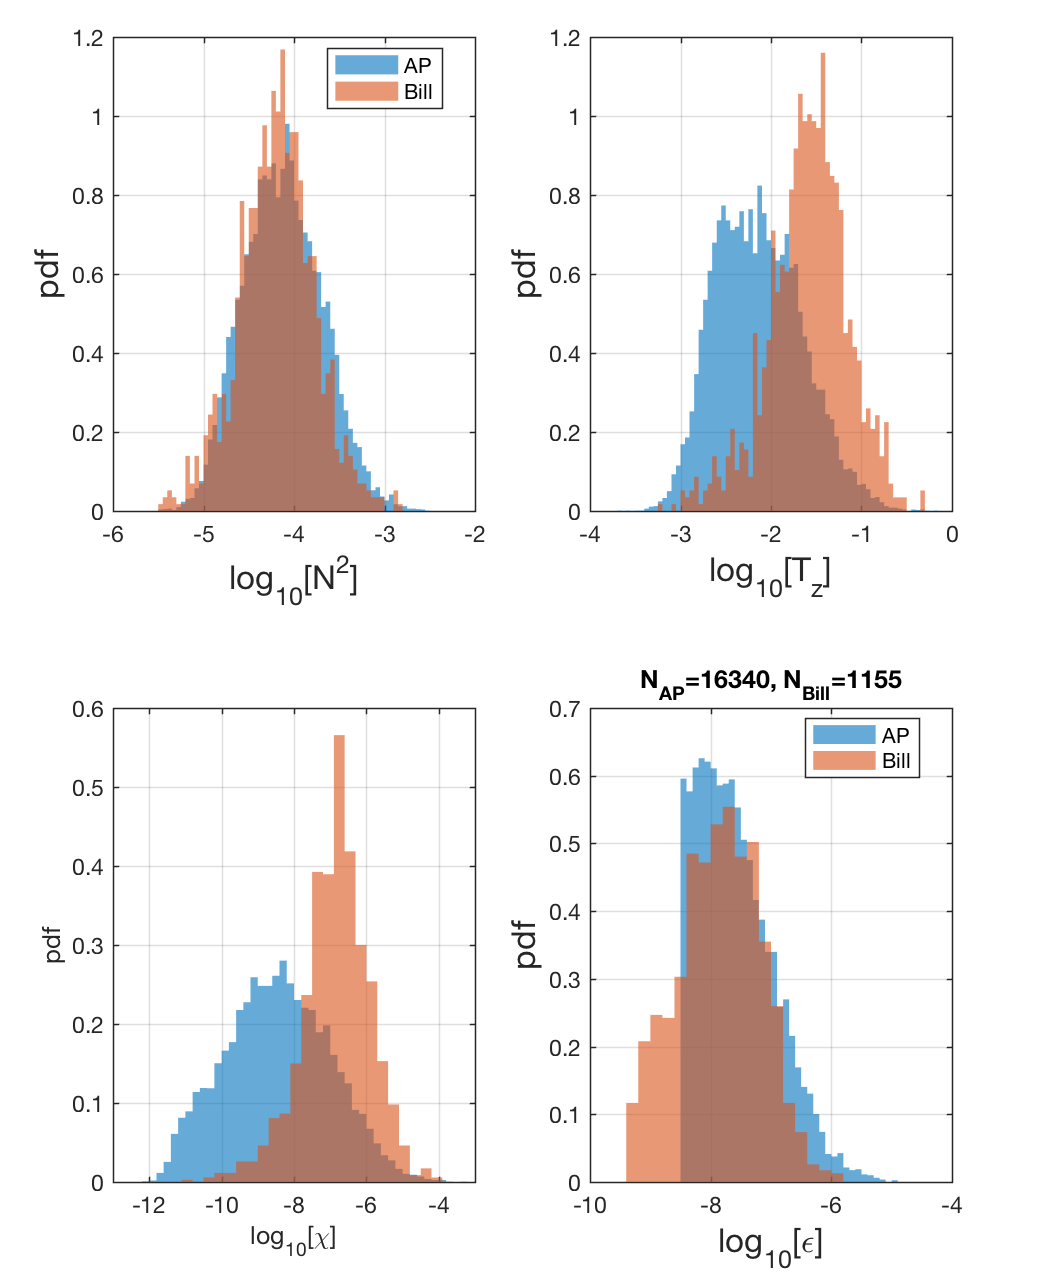
\includegraphics[scale=0.8]{tiwe_minOT_40_usetemp_1_n2_tz_chi_eps_apvsbill_hist_yday_324_327.png}
\caption{Histograms of $N^2$ , $T_z$, $\chi$, and $\epsilon$ for patches analyzed by myself and Bill. Data for profiles on yday 324-327, between 60-200m depth.}
\label{comp_bill_ap_1}
\end{figure}
%

\begin{figure}[htbp]
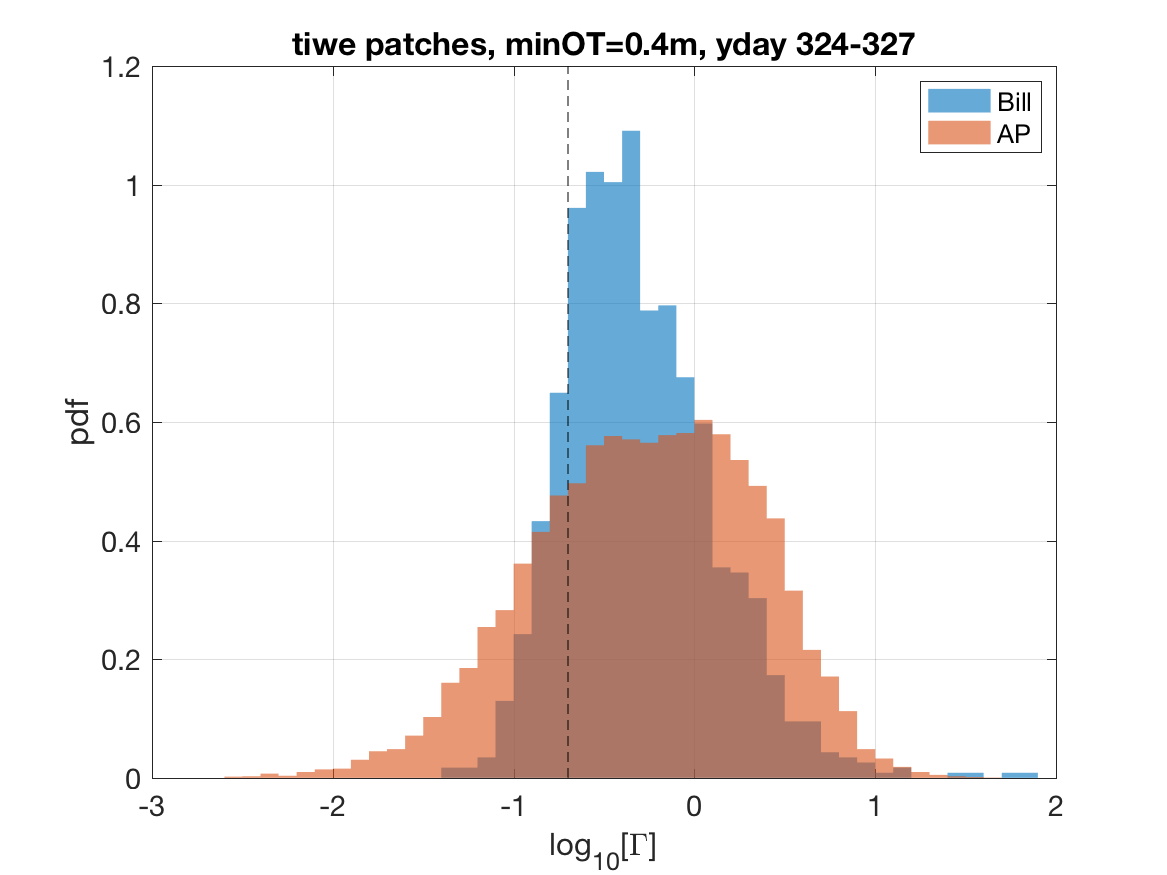
\includegraphics[scale=0.8]{tiwe_minOT_40_usetemp_1_gam_apvsbill_hist_yday_324_327.png}
\caption{Histograms of $\gamma_{\chi\epsilon}$ for patches analyzed by myself (`line' method)  and Bill. Data for profiles on yday 324-327, between 60-200m depth.}
\label{comp_bill_ap_gam}
\end{figure}


%
%\clearpage
%%~~~~~~~~~~~~~~~~
%\subsection{Yday 324-327}
%
%I noticed that in Smyth et al 2001, only data from ydays 324-327 is used for the TIWE patches. So I remade the previous figures using only data from that time period (Figures \ref{comp_bill_ap_324_327},\ref{comp_bill_ap_gam_324_327}). Using this data, I get  gammas centered around 0.2 and close to Bill's estimates. 
%
%\begin{figure}[htbp]
%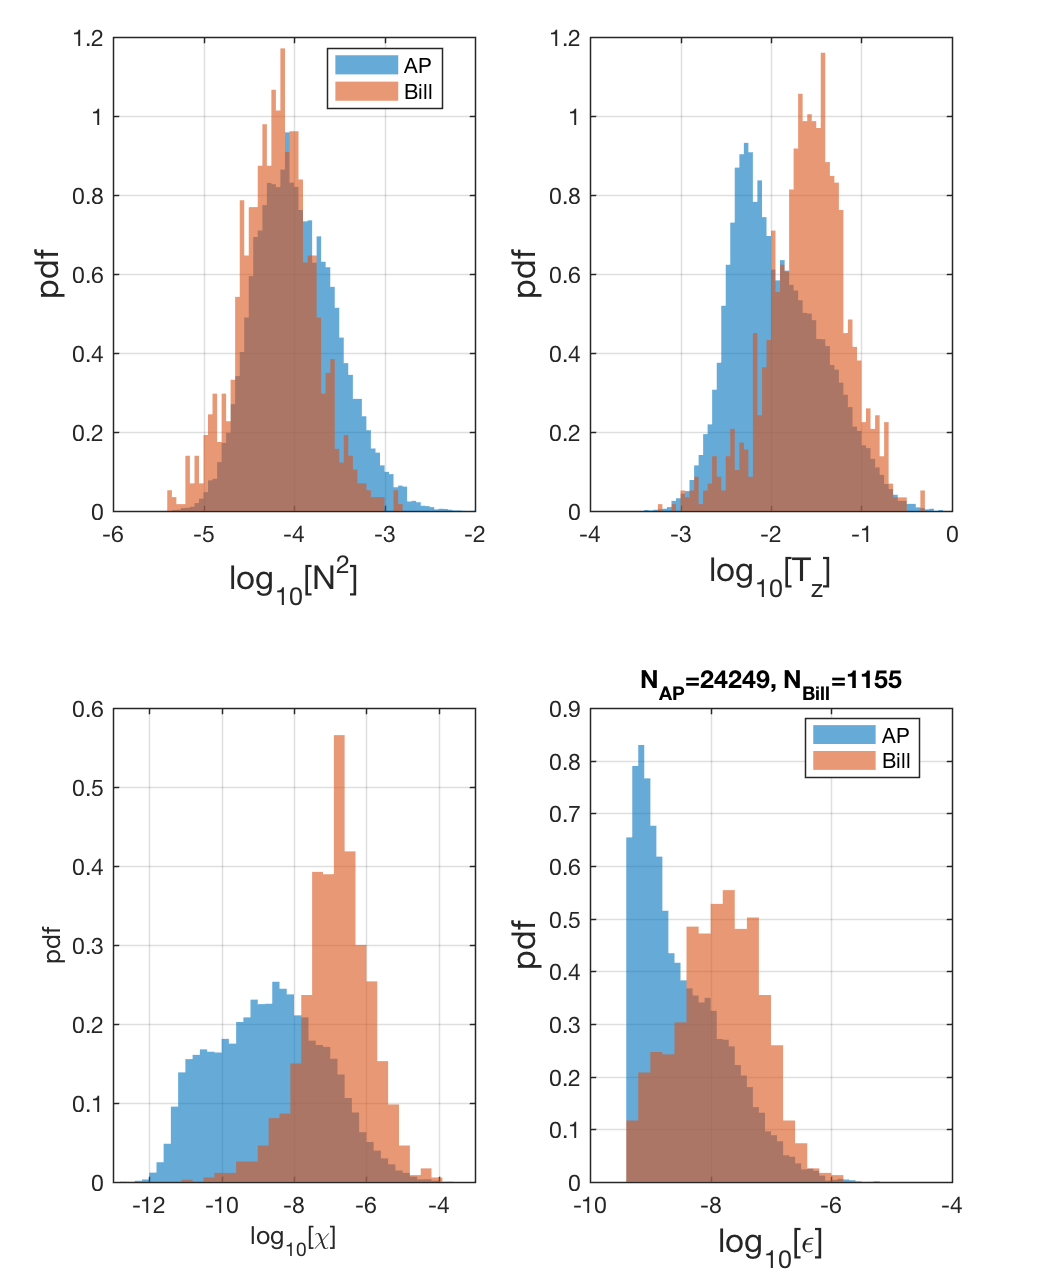
\includegraphics[scale=0.8]{tiwe_minOT_15_usetemp_1_n2_tz_chi_eps_apvsbill_hist_yday_324_327_merged_minsep_15.png}
%\caption{Histograms of $N^2$ , $T_z$, $\chi$, and $\epsilon$ for patches analyzed by myself and Bill. Data for profiles on yday 324-327 (corresponding to data used in Smyth et al).}
%\label{comp_bill_ap_324_327}
%\end{figure}
%
%
%\begin{figure}[htbp]
%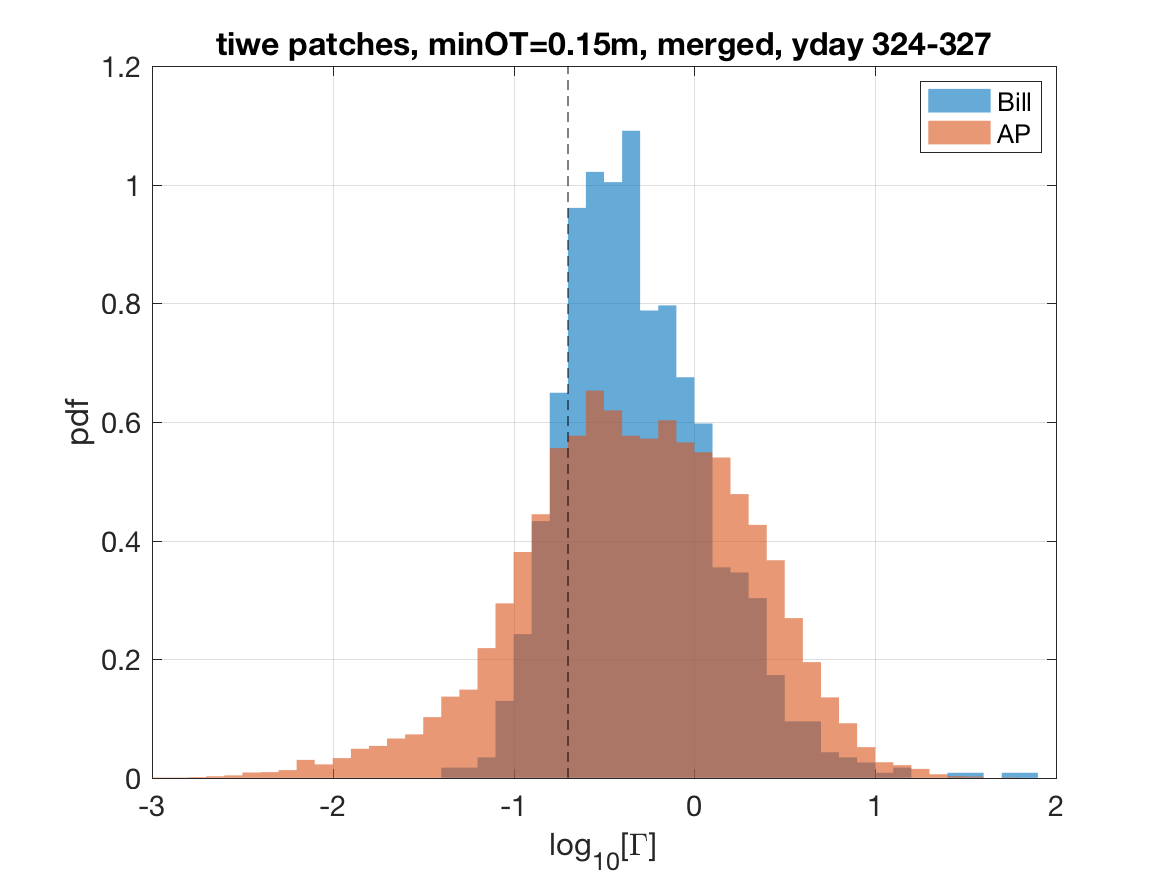
\includegraphics[scale=0.8]{tiwe_minOT_15_usetemp_1_gam_apvsbill_hist_yday_324_327_merged_minsep_15.png}
%\caption{Histograms of $\gamma_{\chi\epsilon}$ for patches analyzed by myself and Bill. Data for profiles on yday 324-327 (corresponding to data used in Smyth et al).}
%\label{comp_bill_ap_gam_324_327}
%\end{figure}





%\newpage
%\clearpage
%%~~~~~~~~~~~~~~~~
%\subsection{To Merge or not to Merge?}
%
%In the Smyth et al 2001 methods section, it says that patches separated by less than 15cm are also merged together. So I tried repeating the analysis with merged patches to see how it affects the results. The raw patches for each profile are merged in \verb+merge_patches_tiwe.m+ .
%


%\begin{figure}[htbp]
%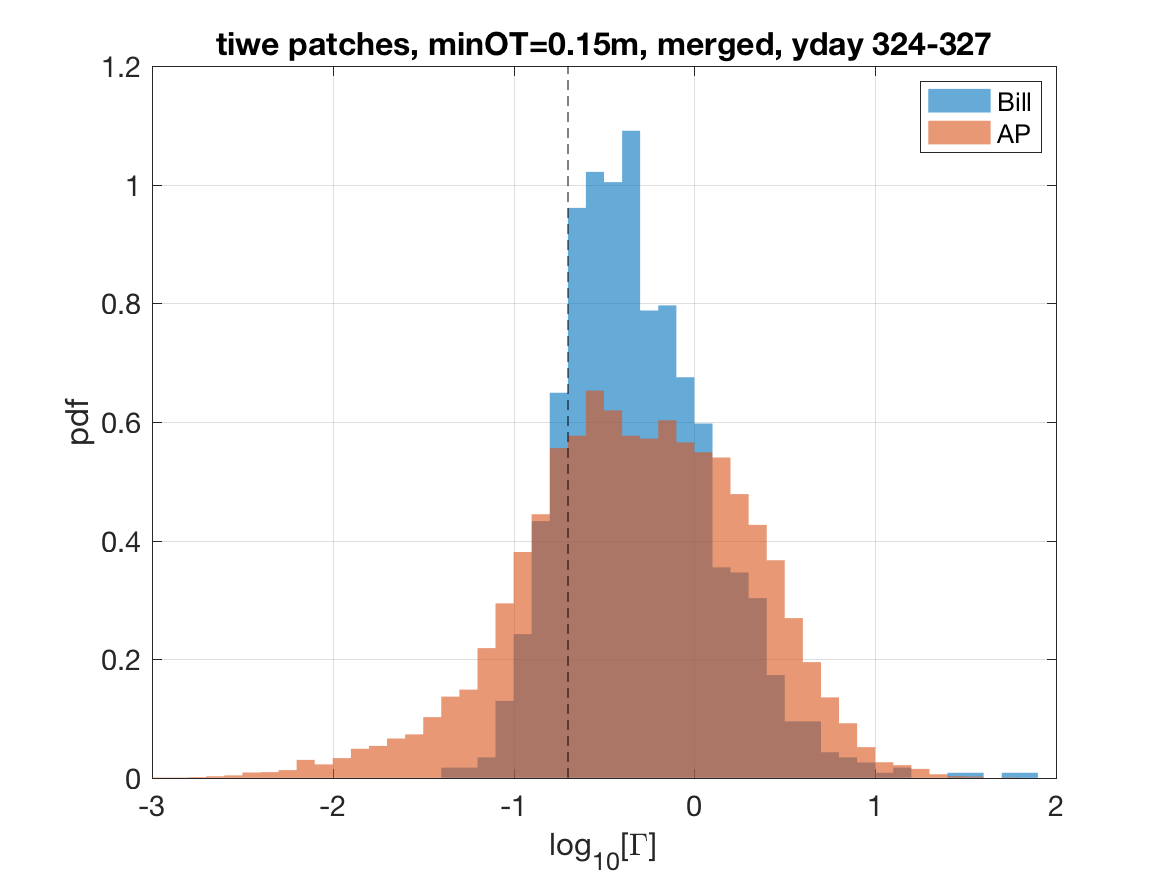
\includegraphics[scale=0.8]{tiwe_minOT_15_usetemp_1_gam_apvsbill_hist_yday_324_327_merged_minsep_15.png}
%\caption{Histograms of $\gamma_{\chi\epsilon}$ for *merged* patches analyzed by myself and Bill. Data for profiles on yday 324-327 (corresponding to data used in Smyth et al).}
%\label{comp_bill_ap_gam_324_327}
%\end{figure}






%
%\clearpage
%%~~~~~~~~~~~~~~~~
%\subsection{Variation of $\gamma_{\chi\epsilon}$ over time}
%
%Since it appears that $\gamma_{\chi\epsilon}$ can vary for different time periods, I wanted to investigate this more. I plotted $\gamma_{\chi\epsilon}$ vs yday (Figure \ref{gamvsyday}). It looks like the median $\gamma_{\chi\epsilon}$ is smaller than 0.2 for ydays less than 315, and then about equal to 0.2 after that (a few days are abnormal and might not have many profiles).
%
%\begin{figure}[htbp]
%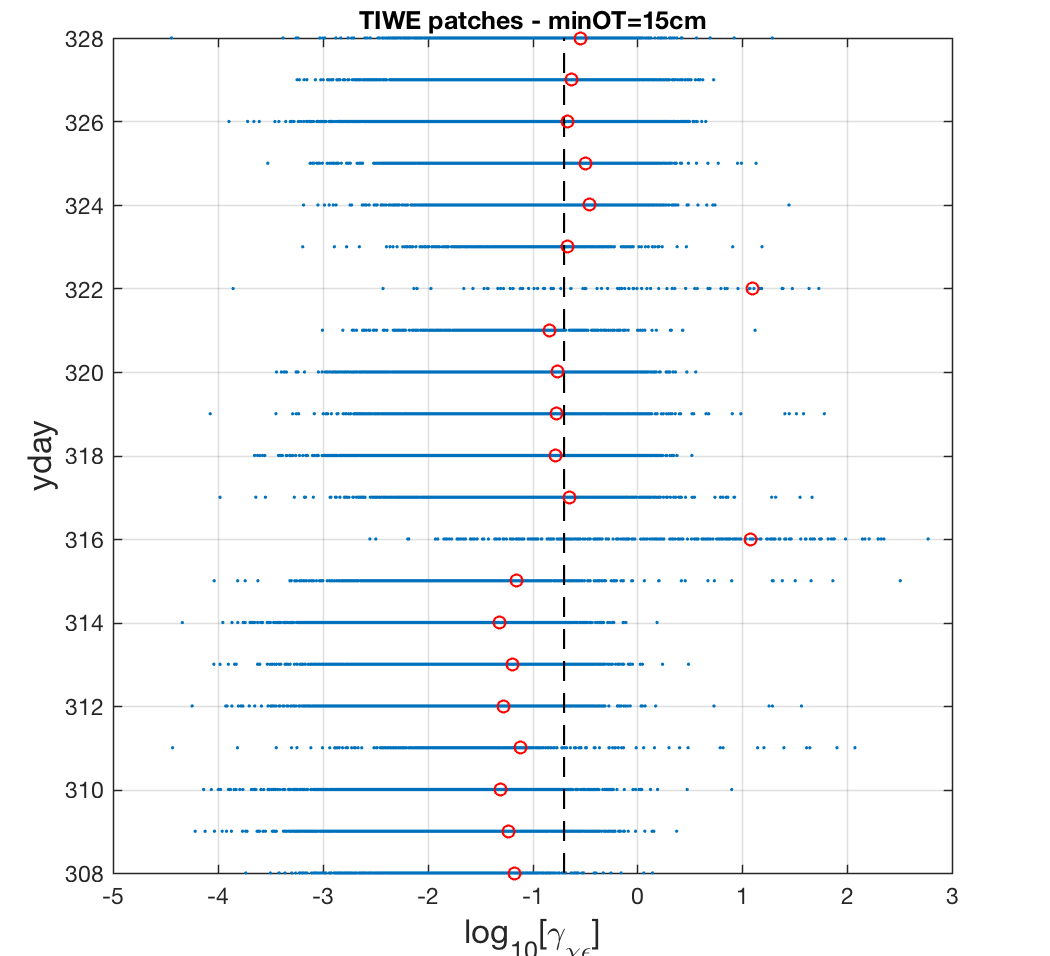
\includegraphics[scale=0.8]{tiwe_minOT_15_usetemp_1_gam_vs_yday.png}
%\caption{Plot of $\gamma_{\chi\epsilon}$ for patches vs yday. Vertical line is $\gamma_{\chi\epsilon}=0.2$. Red circles are the median value for each day. * what happend on yday 322.326?}
%\label{gamvsyday}
%\end{figure}





%~~~~~~~~~~~~~~
\end{document}  


